\documentclass{article}

\usepackage[margin=0.3in]{geometry}
\usepackage{multicol}
\usepackage[T1]{fontenc}
\usepackage{lipsum}
\usepackage{color}
\usepackage{tikz}
\usepackage{amsmath}
\usepackage{graphicx}
\usepackage[usenames, dvipsnames]{color}
\usepackage[linesnumbered,boxed,commentsnumbered,lined]{algorithm2e}
\usetikzlibrary{positioning}

\tikzset{
  gray box/.style={
    fill=gray!20,
    draw=gray,
    minimum width={2*#1ex},
    minimum height={2em},
  },
  annotation/.style={
    anchor=north,
  }
}

\setlength\parindent{0pt}

% Alias for bold small caps
\newcommand{\smallcaps}[1]{\textsc{\textbf #1}\\}

\begin{document}
  \begin{multicols}{2}
    A computer whose processes have 1024 pages in their address spaces keeps
    its page tables in memory. The overhead required for reading a word from
    the page table is 500 nsec.  To reduce this  overhead, the computer has an
    associative  memory  which holds 32 (virtual  page,  physical  page frame)
    pairs and can do look up in 100 nsec.  What hit rate is needed  to reduce
    the mean overhead to 200 nsec?

    \smallcaps{Solution}

    The effective instruction time is $100h + 500(1-h)$, where h is the
    hit rate. $100$ is the look up time \& $500$ is the overhead. Set the
    expression equal to 200 and solve for h. We get h must be 0.75 (or greater).

    \begin{align*}
      100h + 500(1-h) &= 200 \\
      100h + 500 - 500h &= 200 \\
      -400h + 500 &= 200 \\
      -400h &= -300 \\
      h &= \frac{-300}{-400} \\
      h &= \frac{3}{4} \implies 75\%
    \end{align*}

    \section*{Address Translation}
    \begin{tabular}{|c|c|c|}
      \hline
      Frame Number & Process ID & Page Number \\
      \hline
      0 & 1 & 2 \\
      \hline
      1 & 1 & 1 \\
      \hline
      2 & 2 & 1 \\
      \hline
      3 & 3 & 0 \\
      \hline
      4 & 1 & 3 \\
      \hline
    \end{tabular}

    Using the table above, translate the following:

    \begin{enumerate}
      \item To which physical address does virtual address 130 of process 1 map to?
        If this virtual address does not map to any physical address, write `does not map'.
      \item To which physical address does virtual address 17 of process 2 map to?
        If this virtual address does not map to any physical address, write `does not map'.
      \item Which virtual address of which process maps to physical address 50?
    \end{enumerate}

    \smallcaps{Solution}

    \begin{enumerate}
      \item logical $= (1 \times 100) + 30 \implies 130$ \\
        Physical $=$ frame\# $= 1 \implies (1 \times 100) + 30 = 130$
      \item Virtual address 17 does not map
      \item Physical address $= (0 \times 100) + 50 = 50$ Where $0$ is the frame\# \\
        So, logical address $= (2 \times 100) + 50 = 250$ Where $2$ is the page\#
    \end{enumerate}

    \section*{File system implementation}
    Consider a File system that maintains unique index node for each
    file in the system. Each index node includes 10 direct pointers, a single indirect pointer,
    and a double indirect pointer. The file system block size is 1024 bytes, and a block pointer
    occupies 4 bytes.

    \begin{enumerate}
      \item What is the maximum file size that can be supported by the index node?
      \item How many disk operations will be required if a process read data from the $N^{th}$ block
        of a file? Assume that the file is already open, the buffer cache is empty, and each disk
        operation read a single file block. Your answer should be given in terms of $N$.
    \end{enumerate}

    \smallcaps{Solution}

    \begin{enumerate}
      \item $1024 * (10 + 2^8 + 2^8 * 2^8)$ \\
        $\implies 2^{10} * (2^3 + 2 + 2^8 + 2^{16})$ \\
        $\implies 2^{13} + 2^{11} + 2^{18} + 2^{26}$ \\
      \item $0 \le N < 10$, One operation \\
        $10 \le N < 256 + 10$, Two operations \\
        $256 + 10 \le N < 2^{13} + 2^{11} + 2^{18} + 2^{26}$, Three operations
    \end{enumerate}

    \# 6 part c:
    \begin{itemize}
      \item $1 \le N < 10$, One operation
      \item $10 \le N$, $1 + ceiling(\frac{n - 10}{255})$
    \end{itemize}

    Allocations

    \begin{itemize}
      \item Contiguous Allocation : Each file occupies a set of contiguous blocks on the disk.
      \item Linked Allocation : Each file is a linked list of disk blocks: blocks may be scattered
        anywhere on the disk.
      \item Indexed Allocation : Brings all pointers together into the index block.
    \end{itemize}

    \section*{Disk Scheduling}

    \begin{itemize}
      \item First-come, First-served: the requests are processed in the order they were received.
      \item Shortest Seek Time First: Process the request that is closest to the arms current
        position.
      \item SCAN: Process all the requests going in one direction until they are complete, and then
        change the direction of the arm and process the rest of the requests.
      \item C-SCAN: Process all the requests going in one direction. When arm reaches the end, start
        back at the beginning and finish out the rest of the requests.
      \item C-LOOK: Process all the requests in one direction, when the last request in that direction
        is completed, change the direction of the arm and process the rest of the requests in the
        other direction.
    \end{itemize}

    \section*{Page Replacement Algorithms}

    \begin{itemize}
      \item First-in First-out (FIFO): when a page must be replaced, the oldest page is chosen.
      \item Optimal: Replace page that will not be used for the longest period of time.
      \item LRU: Replace the page that has not been used for the longest period of time.
    \end{itemize}

    \section*{Deadlock}

    Four conditions for deadlock:
    \begin{itemize}
      \item Mutual Exclusion
      \item Hold and Wait
      \item No Preemption
      \item Circular Wait
    \end{itemize}

    For calculating the needs matrix, we take maximum $-$ current. To derive the safe order, We
    start with the initial work, and we check the current allocation and if that is less than the
    current work, that process is added to safe state \& then we add the current allocation to the
    work available.

    \section*{Segmentation}

    A virtual memory system supports 12 bits length virtual addresses. It uses pure segmentation
    with a maximum segment size of $2^{10}$ (1024) bytes. Suppose that the segment table for the
    currently running process looks as follows:

    \begin{tabular}{|c|c|c|c|c|}
      \hline
      Segment \# & V & P & Start & Length \\
      \hline
      0 & 1 & 1 & 0 & 200 \\
      \hline
      1 & 1 & 0 & 1000 & 160 \\
      \hline
      2 & 0 & 0 & 0 & 0 \\
      \hline
      3 & 1 & 0 & 200 & 300 \\
      \hline
    \end{tabular}

    In the table above V and P are the segment `valid' and `protection' bits, `start' represents the
    physical address of the start of the segment and `Length' is the segments's length. $P = 1$
    indicates that a segment is read-only.

    Consider the following read and write operations. If the specified operation would succeed given
    the segment table shown above, give the physical address to which the specified virtual address
    would translate. If it would not succeed, state the reason that it would fail.

    \begin{enumerate}
      \item A write to virtual address 150
      \item A read from virtual address 1025
      \item A write to virtual address 400
    \end{enumerate}

    \smallcaps{Solution}

    \begin{enumerate}
      \item
        $150 = (0 \times 1024) + 150$ \\
        $150 < 200$ \\
        This would fail because there is a protection bit $\implies$ read-only.
      \item
        $1025 = (1 \times 1024) + 1$ \\
        $1 < 1160$ \\
        Physical address $= 1001$.
      \item
        $4000 = (3 \times 1024) + 928$ \\
        $928 > 500$ \\
        This would fail because of a trap: Addressing error.
    \end{enumerate}

    \section*{Buddy Algorithm}
    \begin{center}
      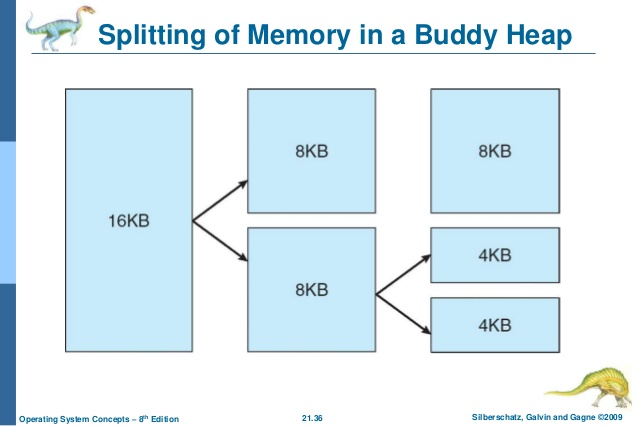
\includegraphics[scale=0.4]{buddy_algorithm.png} \\
    \end{center}

    This would represent a request for $<$ 4KB. In the example above one of the 4KB blocks would be
    allocated to the current request.

    Internal fragmentation is wasted memory visible only to the process making the memory request.
    Internal fragmentation occurs in buddy allocation because memory requests must be rounded up to
    the nearest power of 2.

    So, for example if we had a request of 2KB, then the internal fragmentation would be $4KB - 2KB
    = 2KB$

    External fragmentation is wasted memory visible to the system outside of the requesting
    processes. External fragmentation occurs because not all requests (even after they've been
    rounded up to the nearest power of two) are the same size; therefore, it is possible that a
    memory request will not be able to satisfied, even when there is enough total free memory in the
    system.

    Basically: External fragmentation is because it's not contiguous.
  \end{multicols}
\end{document}
